\documentclass[12pt]{article}
\usepackage{amsmath}
\usepackage{graphicx}
\DeclareGraphicsExtensions{.pdf,.png,.jpg}

\newtheorem{theorem}{Theorem}[section]
\newtheorem{lemma}[theorem]{Lemma}
\newtheorem{definition}[theorem]{Definition}


\title{Differential Drive}
\date{}
\begin{document}
  \maketitle
  
  \section{Five Strategies of Diff Drive}
  
  Consider start configuration $q_{s} = (x,y,\theta)$ and goal configuration $q_{g} = (0,0,0)$, where $\theta \in [0, \frac{\pi}{2}]$. We can partition them into 8 partitions.
  
  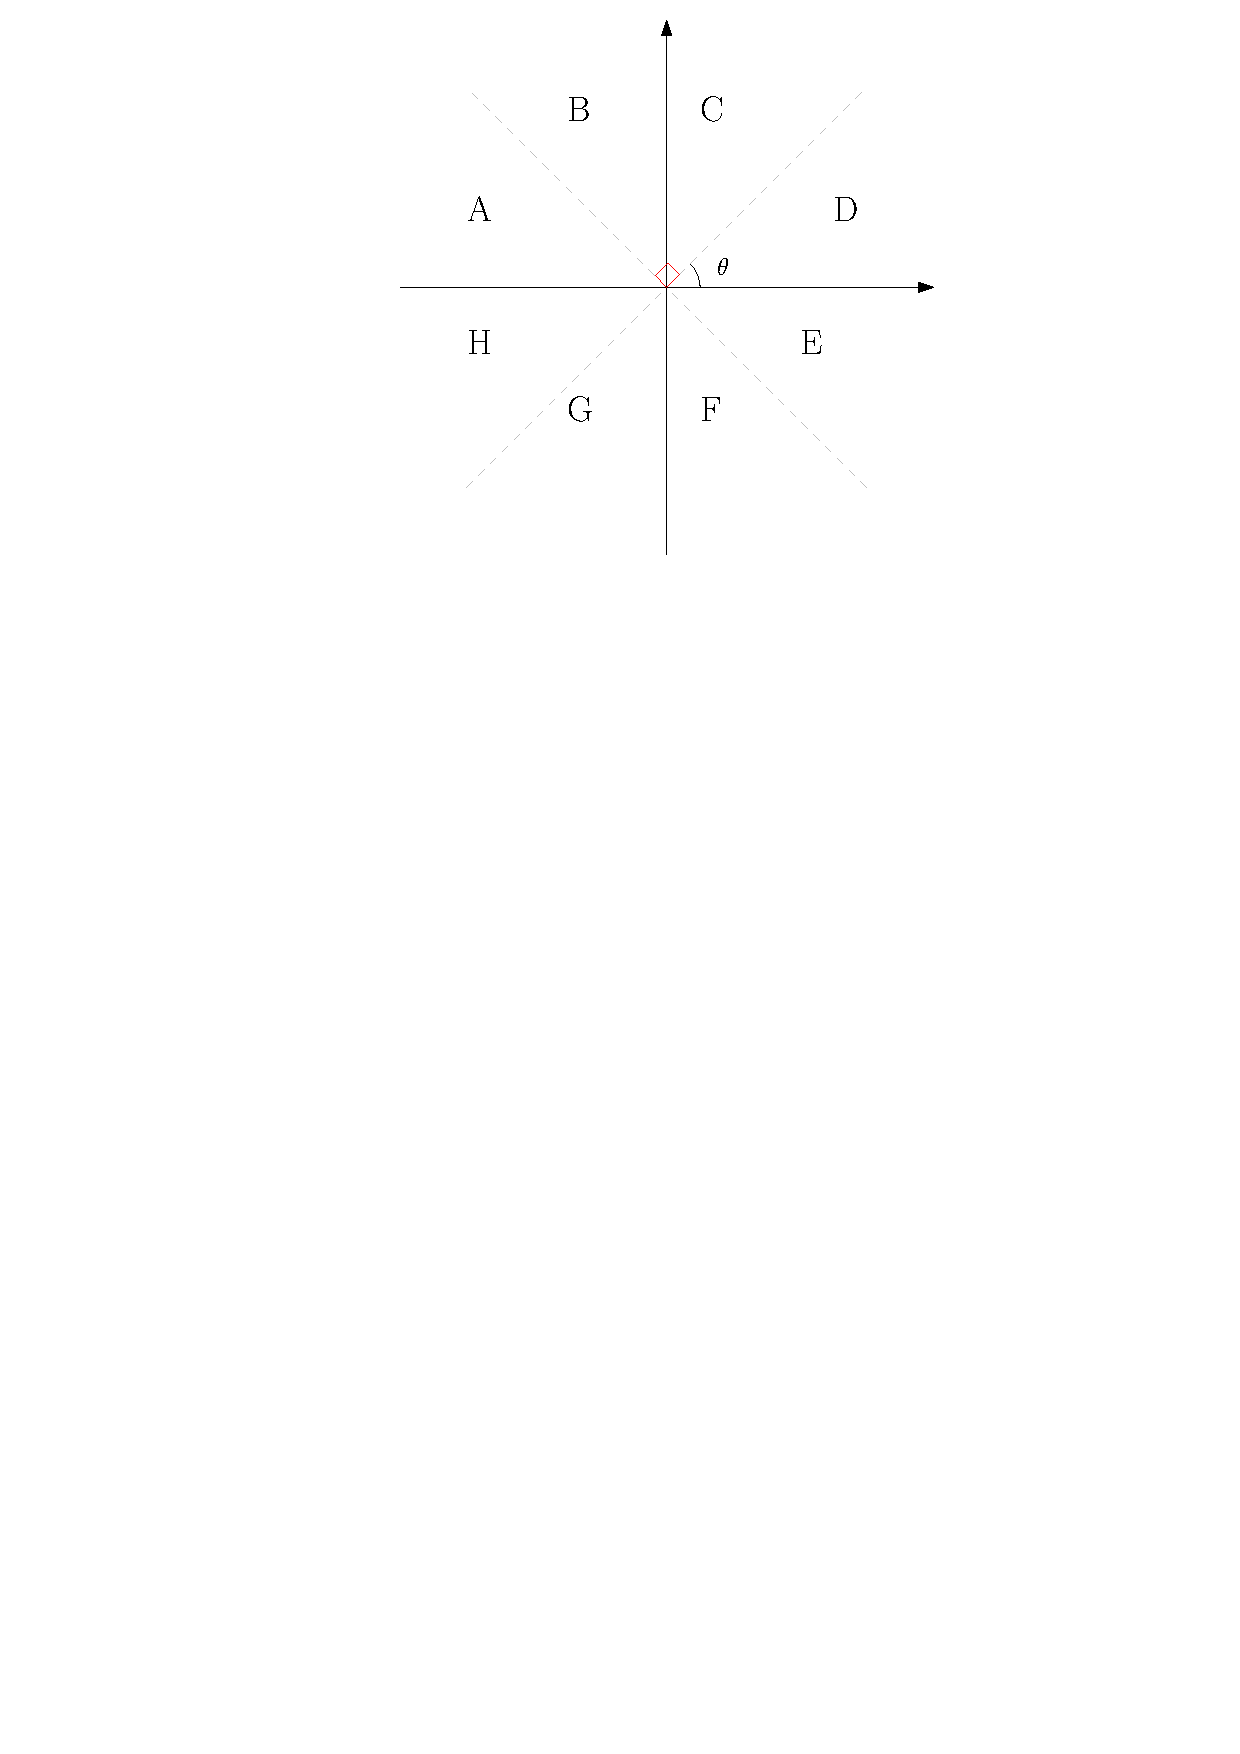
\includegraphics{Coordinate}\\
  
  In the next 5 subsections, we will provide different path's for a diff drive to reach goal config when start position is in different partitions. 
  
  Green arrow, in the graphs, means the start orientation while red arrow means the goal orientation. Black arrows imply the orientation at the point. Black lines or arcs are the path a diff drive will go through. Gray lines are assistant lines for analyzing the cost.  Every (circular) arc is 90 degree.\\
  
  Denote arc path as A, straight path as S and turn to be T. \\  
  
  Partition H and D:
  
  The optimal path in these situations is known. $\cite{devin}$ proved the strategy to be "Turn-Drive-Turn". Written as T-S-T with our notation. 
  
  The cost in this case is $|SG|+g(\theta)$, where $g(\theta)$ is the minimum cost for turning the car. 
  \\
  
  Partition A:
  
  \begin{figure}
  \centering
  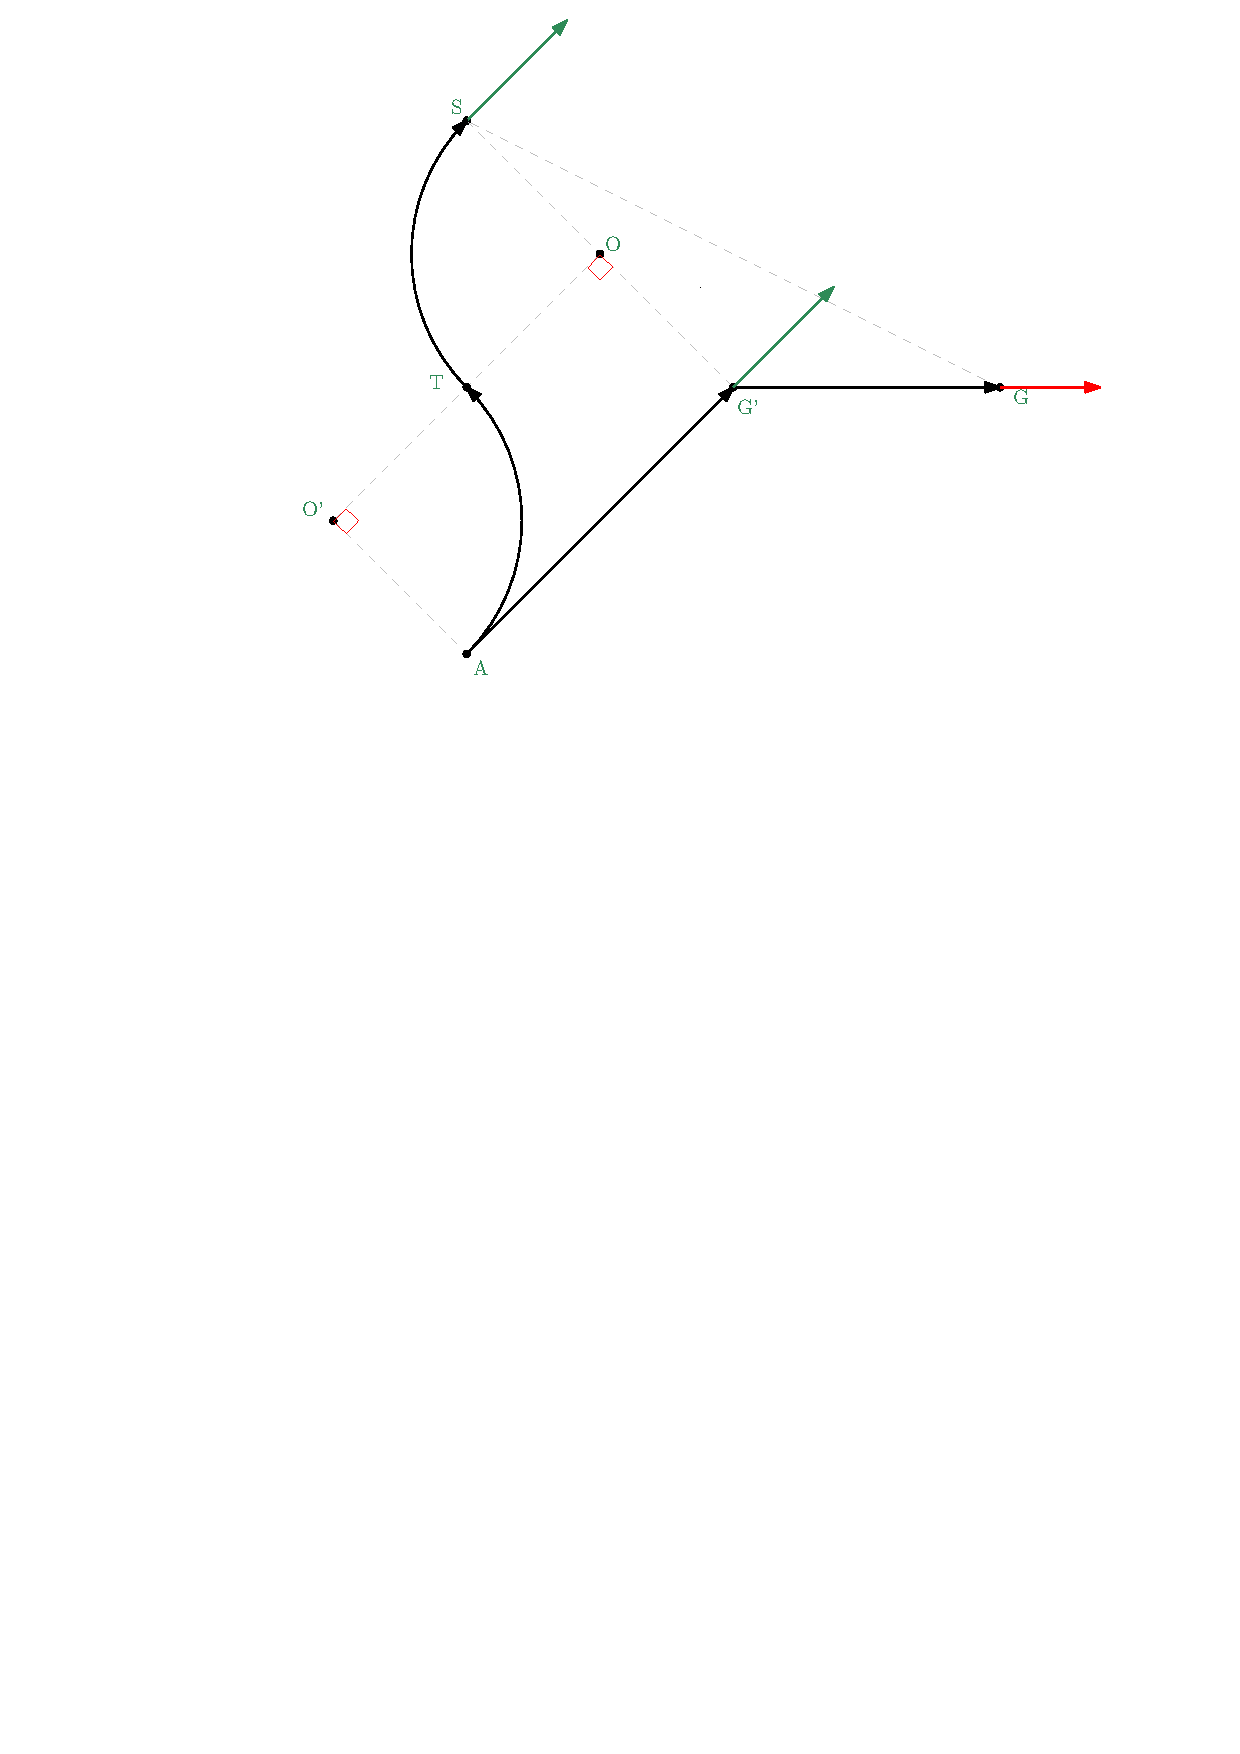
\includegraphics[scale=0.65]{Diff_Drive_Gene_Case_4}
  \caption{Path when start position S is in partition A. }
  \end{figure}
  
  The path in this case is A-A-S-T-S. (see fig 1)
  
  The cost will be: 
  
  $C = (\frac{\pi}{2}+1)|SG'| + |G'G| + g(\theta)$\\
  
  $|SG'| = \frac{y}{cos( \frac{\pi}{2} - \theta )};    |G'G| = \frac{y}{sin( \frac{\pi}{2} - \theta )}$\\
  
  $C = (\frac{\pi}{2}+1) \cdot•\frac{y}{cos( \frac{\pi}{2} - \theta )} + \frac{y}{sin( \frac{\pi}{2} - \theta )} + g(\theta) $\\

  Partition B and C:
  
  \begin{figure}
  \centering
  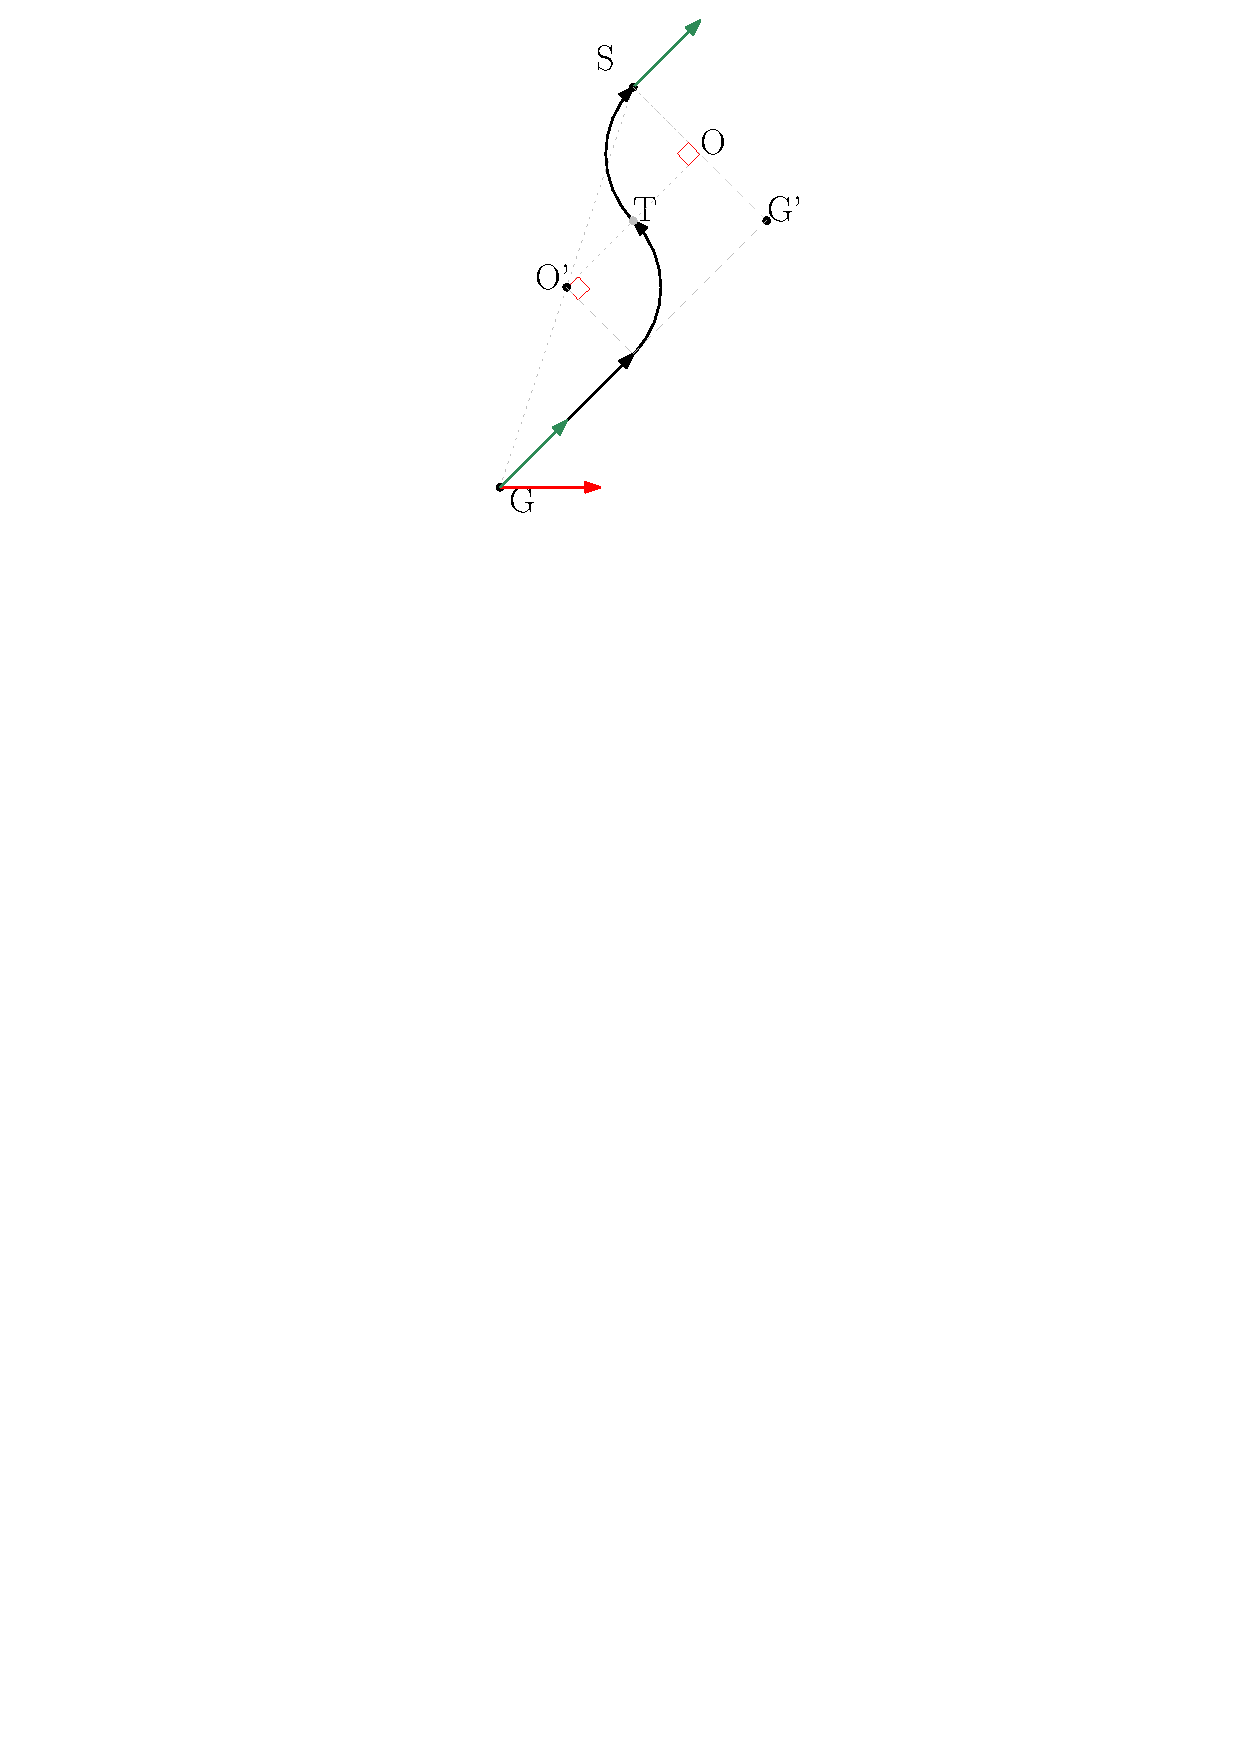
\includegraphics[scale=1]{Diff_Drive_Gene_Case_3}
  \caption{Path when start position S is in partition B or C.}
  \end{figure}
  
  The path is S-A-A-T. (see fig 2)\\
  
  Partition E:
  
  \begin{figure}
  \centering
  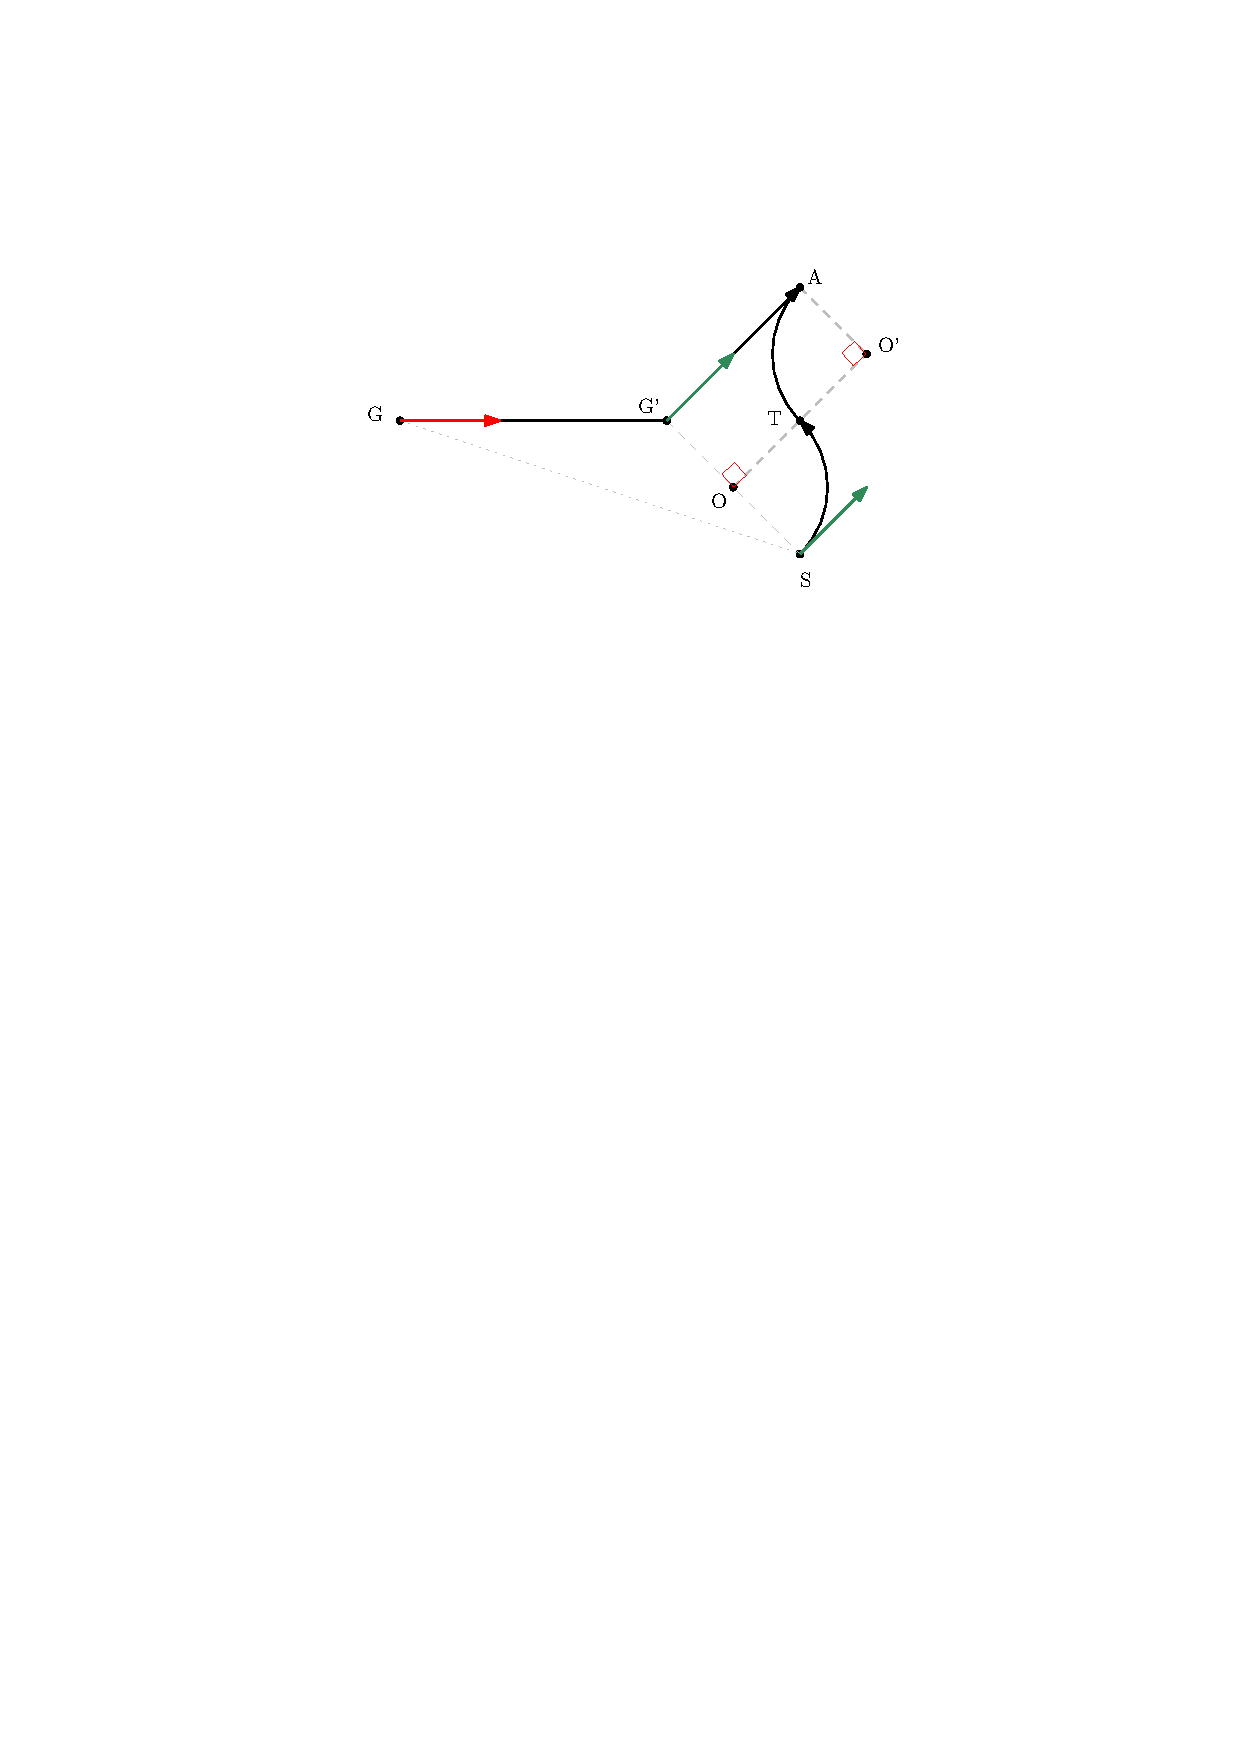
\includegraphics[scale=1]{Diff_Drive_Gene_Case_2}
  \caption{Path when start position S is in partition E.}
  \end{figure}

  The path is A-A-S-T-S. (see fig. 3)\\

  Partition F and G:
  
  \begin{figure}
  \centering
  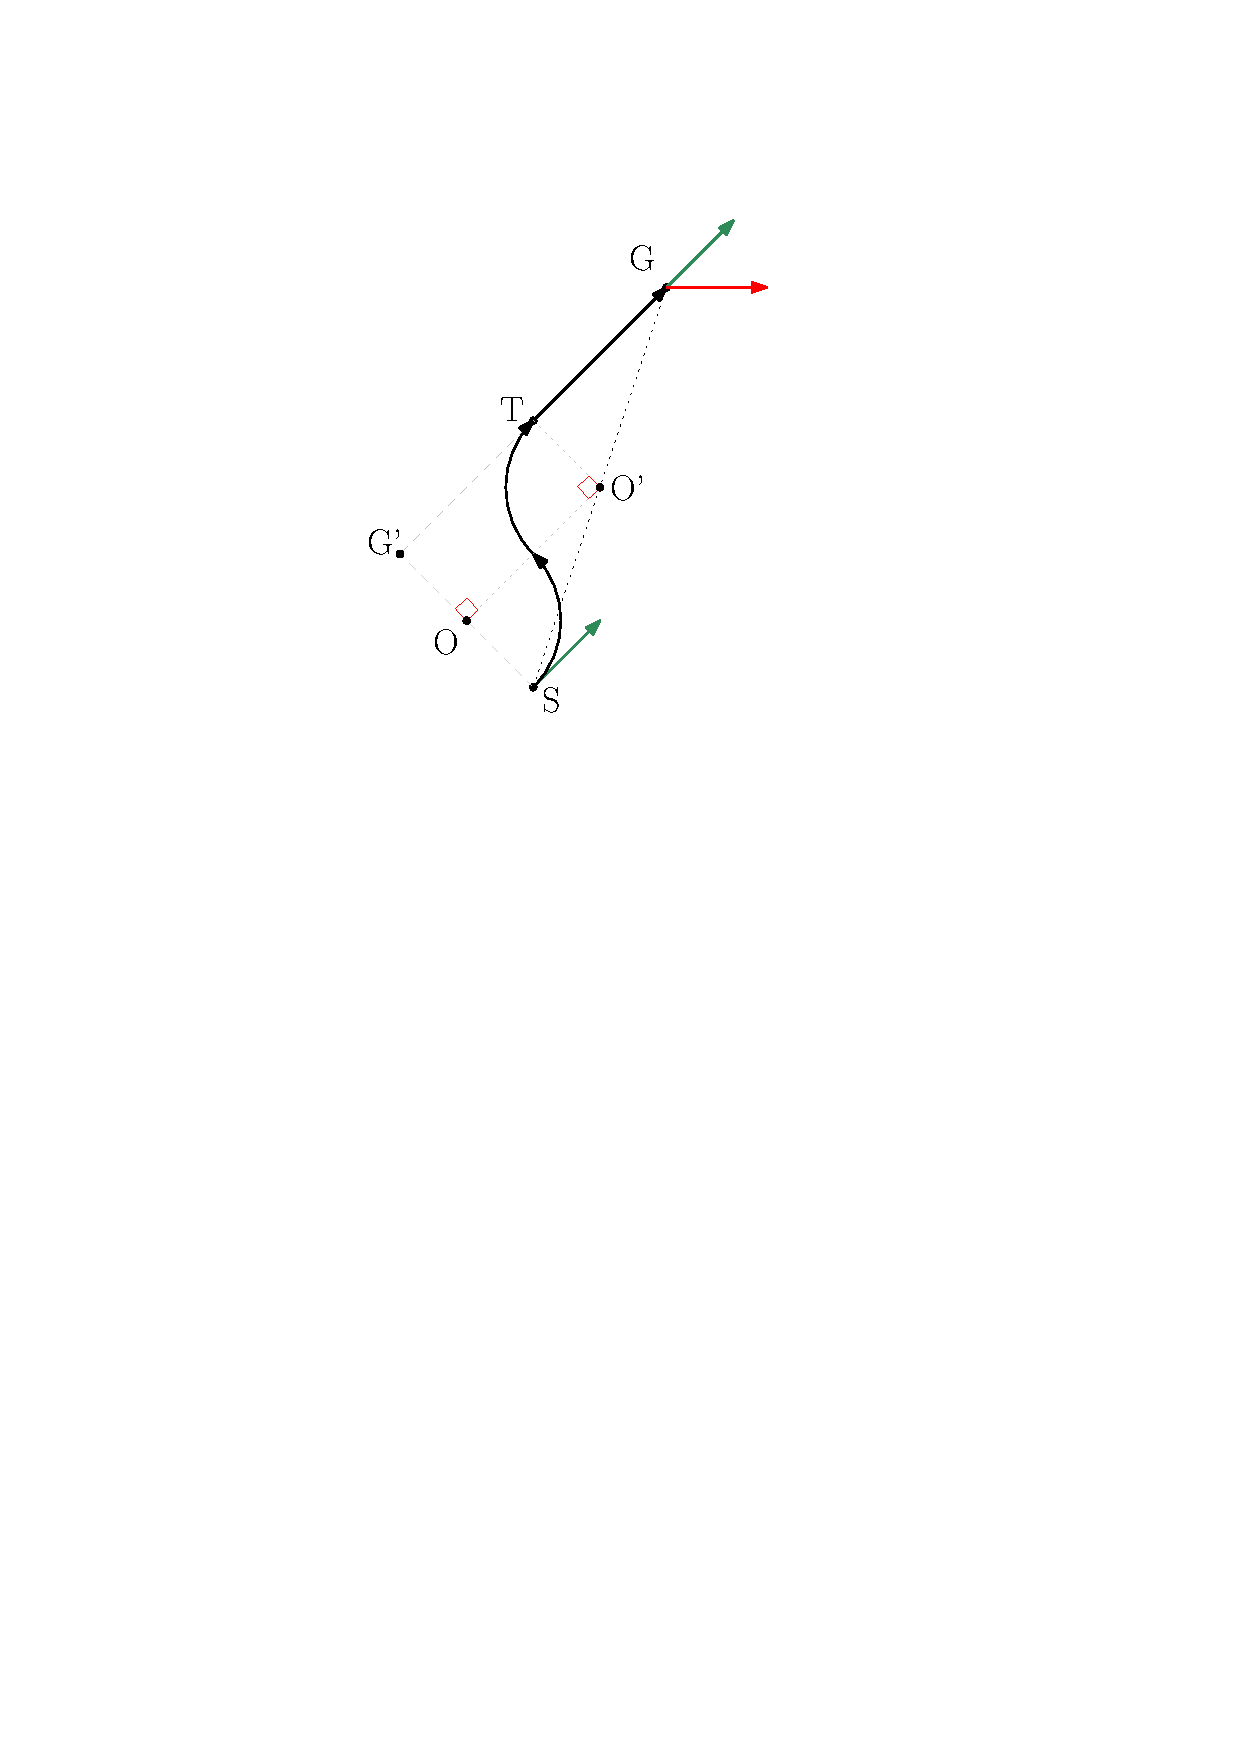
\includegraphics[scale=1]{Diff_Drive_Gene_Case_1}
  \caption{Path when start position S is in partition F or G.}
  \end{figure}
  
  The path is A-A-S-T. (see fig. 4)\\
  ffda
  \subsection{Cost and The Worst Cost}

  \begin{theorem}
  	For a start configuration $q_{s} = (x_{s},y_{s},\theta)$, a goal configuration $q_{g} = (x_{g},y_{g},\theta)$ and a path $\sigma$ with length $l$. $\sigma$ cannot be the optimal path if $l > (\frac{\pi}{2} + 1) \cdot d$, where $d$ is the Euclidean distancce between start and goal position in work space.
  \end{theorem}

  Since the path's above guarantee the diff drive to reach the goal configuration. The cost of these path's can be view as upperbound cost of optimal path. Any path with cost larger than this cannot be optimal. \\
  
  Let $q_{s} = (x,y,\frac{\pi}{3})$ and $q_{g} = (0,0,0)$. The cost can be shown in the image below:
  
  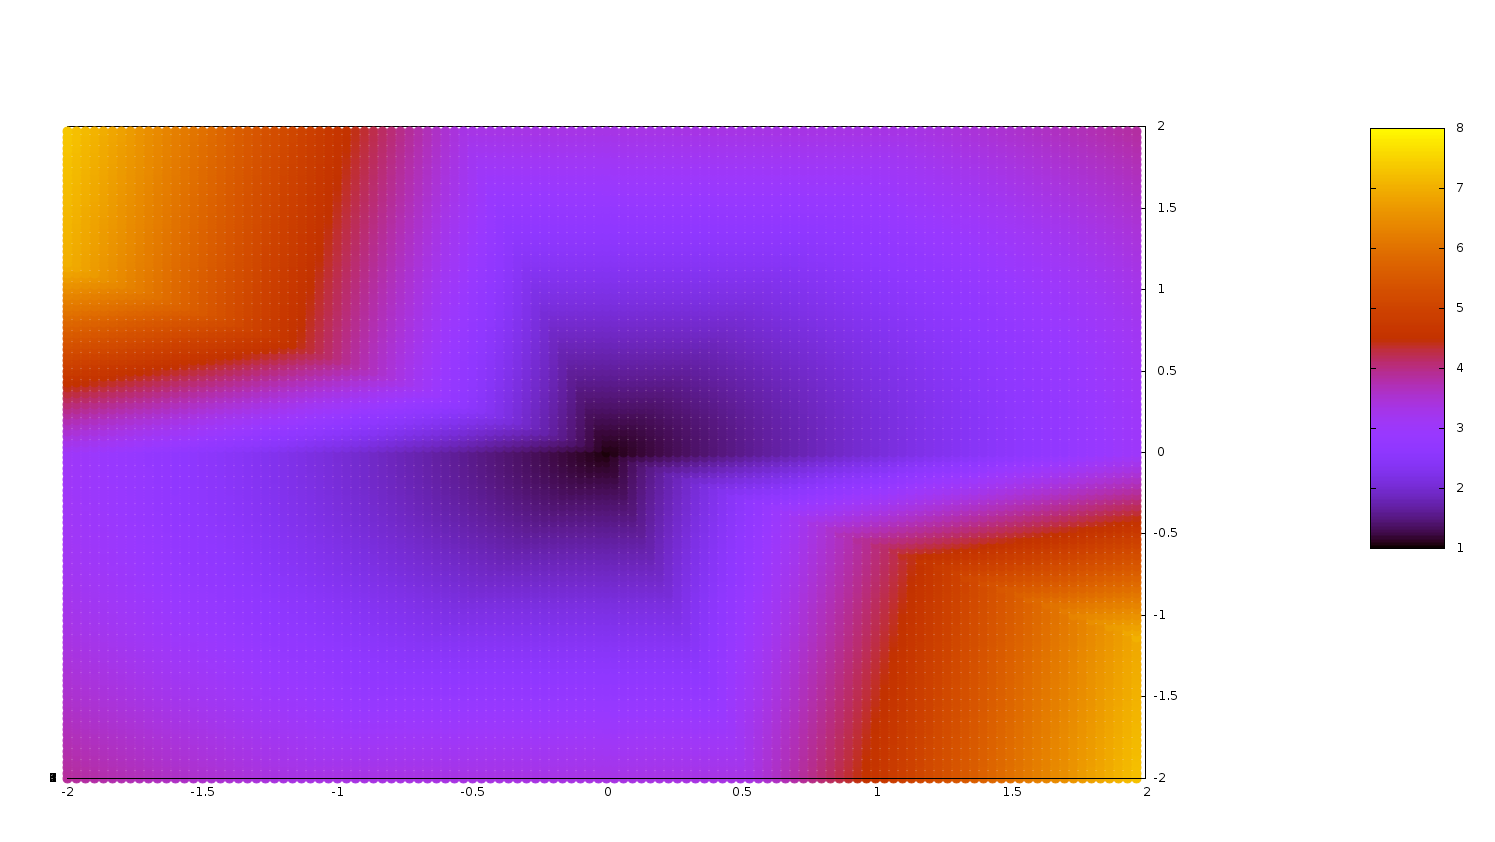
\includegraphics[scale=0.27]{CostImage}\\
  
  Except for the situation that start position is in H or D partition, all other situations have the same maximun cost. When the start orientation is perpendicular to the line segment connection start and goal position.\\
  
  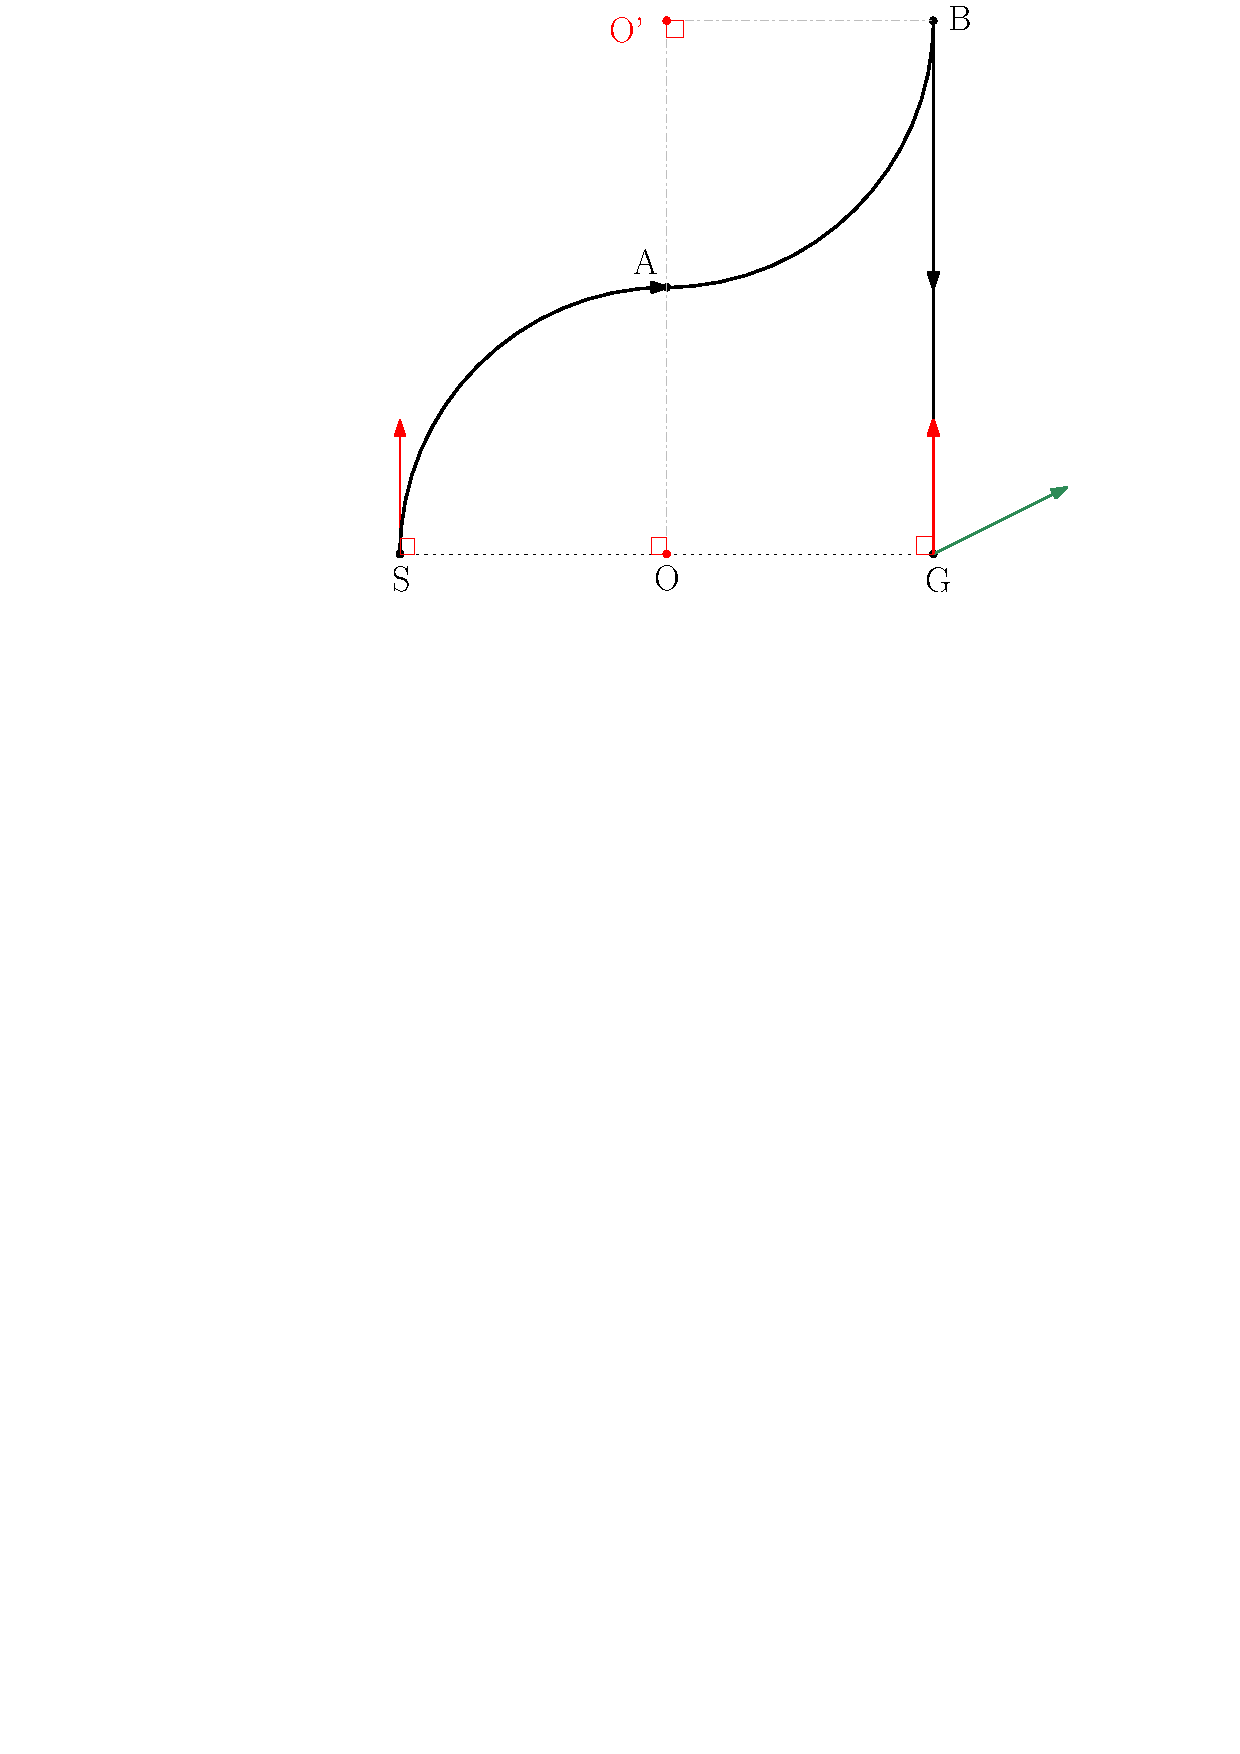
\includegraphics[scale=0.8]{Diff_Drive_Worst_Case}\\
  
  In the worst case, the cost is $C = (\frac{\pi}{2} + 1) \cdot d + g(\theta)$. If start and goal configs have the same orientations, $g(\theta) = 0$, meaning that a diff drive can have a path no longer than $(\frac{\pi}{2} + 1) \cdot d$.
  
  \section{Optimal Path Upper Bound}
  %---------------------------------------------------------------------------
  % Theorem about the turning angle and min path length to turn such an angle.
  %---------------------------------------------------------------------------
  \begin{theorem}
  	The maximum time for a diff drive to go from one config to another is $Whatever$.
  \end{theorem}
  
  %---------------------------------------------------------------------------
  % Theorem about the upper bound of a path being optimal.
  %---------------------------------------------------------------------------
  \begin{theorem}
  	For a start configuration s = $(x_{s},y_{s},\theta_{s})$, a goal configuration g = $(x_{g},y_{g},\theta_{g})$ and a path $\sigma$ with length $l$. $\sigma$ cannot be the optimal path if $l > r_{min}\pi + |SG|$, where S and G are $(x_{s}, y_{s})$ and $(x_{g}, y_{g})$.
  \end{theorem} 
  
  
  
  %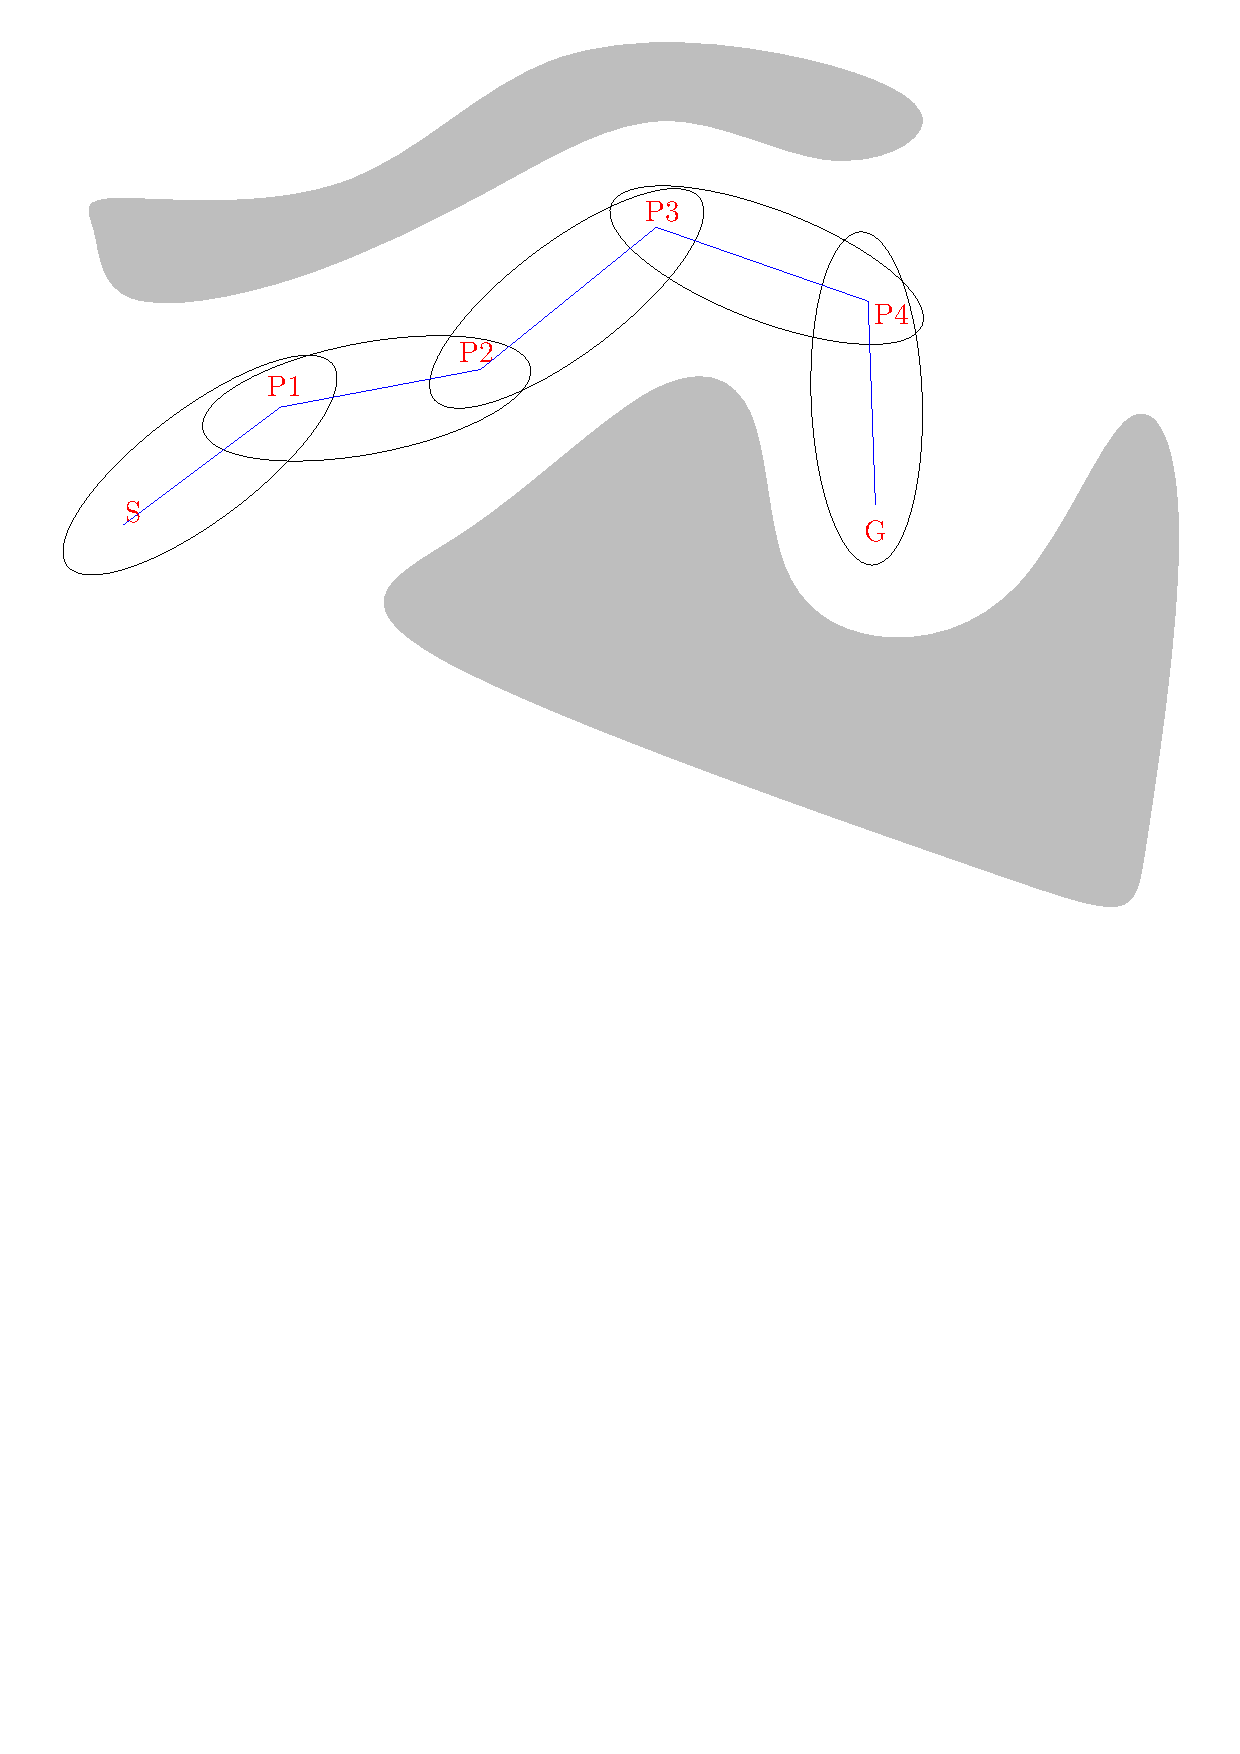
\includegraphics[scale=0.6]{path}\\
  
  
  \begin{thebibliography}{1}

  \bibitem{devin} Balkcom, Devin J., and Matthew T. Mason. "Time optimal trajectories for bounded velocity differential drive vehicles." The International Journal of Robotics Research 21.3 (2002): 199-217.

  \end{thebibliography}
  
\end{document}


